\documentclass[11pt]{article}

\usepackage[margin=1in]{geometry}
\usepackage{amsmath, amssymb}
\usepackage{graphicx}
\usepackage{booktabs}
\usepackage{hyperref}
\usepackage{caption}

\title{Fixed-Embedding Experiment: Does Embedding Geometry\\
       Determine Transformer Performance?}
\author{Claude \& C. L.}
\date{\today}

\begin{document}
\maketitle

%----------------------------------------------------------------------
\section{Motivation}
%----------------------------------------------------------------------

In the cylinder graph HMM setup, the vocabulary has $|V| = 48$ tokens
embedded in $d_{\mathrm{model}} = 8$ dimensions---a 6:1 overcomplete
ratio.  The learned embedding matrix $W_E \in \mathbb{R}^{48 \times 8}$
(tied with the unembedding $W_U = W_E^\top$) is trained jointly with all
transformer blocks.  Analysis of trained models
(cf.\ \texttt{cylinder\_hmm\_model\_comparison.tex}) reveals that $W_E$
consistently develops a $3 \times 3$ block structure in cosine
similarity, mirroring the three depth-level clusters.

This raises a question: \emph{is the specific learned embedding geometry
essential, or does any reasonable embedding suffice?}  If the
transformer blocks are powerful enough to compensate, then freezing $W_E$
at initialisation should incur little loss.  Conversely, if the
embedding geometry is critical, then poorly initialised embeddings will
create an irreducible performance gap.

%----------------------------------------------------------------------
\section{Experimental Conditions}
%----------------------------------------------------------------------

We freeze the embedding $W_E$ and unembed $W_U = W_E^\top$ at
initialisation and train only the transformer blocks (attention layers,
MLP layers, and any bias terms).  Five initialisation strategies are
compared:

\begin{enumerate}
  \item \textbf{Trained} (\texttt{trained}).
    Load $W_E$ from a fully trained checkpoint.  This is the
    \emph{oracle} condition: the embedding already has the ``correct''
    geometry.  Any performance gap relative to the jointly-trained
    baseline reflects the cost of freezing per se (e.g.\ the inability
    to fine-tune embedding norms or small rotations).

  \item \textbf{Random unit-norm} (\texttt{random}).
    Each row of $W_E$ is drawn i.i.d.\ from $\mathcal{N}(0, I_d)$ and
    normalised to the unit sphere $S^{d-1}$.  In $d = 8$ dimensions,
    random unit vectors are approximately orthogonal (expected pairwise
    cosine similarity $\approx 0$), so tokens are roughly equidistant in
    embedding space with no cluster structure.

  \item \textbf{Coulomb (Thomson problem)} (\texttt{coulomb}).
    Place 48 points on $S^7$ by minimising the Coulomb energy
    \begin{equation}
      E = \sum_{i < j} \frac{1}{\|\mathbf{x}_i - \mathbf{x}_j\|},
    \end{equation}
    via gradient descent with projection back onto the sphere after each
    step.  This produces the most uniformly spaced configuration on
    $S^7$, maximising the minimum pairwise distance.  Like \texttt{random},
    this has no cluster structure, but the spacing is deterministic and
    maximally uniform.

  \item \textbf{Sparse binary} (\texttt{sparse\_binary}).
    Each row has $k$ entries set to 1 (at random positions) and the rest
    set to 0, then normalised to unit norm.  With $k = 3$, there are
    $\binom{8}{3} = 56 > 48$ distinct patterns, so all rows can be
    unique.  The resulting embedding is sparse and combinatorial,
    providing a discrete ``code'' for each token.

  \item \textbf{PMI-based (SVD)} (\texttt{pmi}).
    Compute the positive pointwise mutual information (PPMI) matrix from
    sliding-window co-occurrence statistics of the training data:
    \begin{equation}
      \mathrm{PPMI}(i, j) = \max\!\bigl(
        \log \tfrac{P(i,j)}{P(i)\,P(j)},\; 0
      \bigr).
    \end{equation}
    Then take the truncated SVD:
    $\mathrm{PPMI} \approx U \Sigma V^\top$, and set
    $W_E = U_{:,:d} \,\Sigma_{:d}^{1/2}$.
    This embedding directly encodes the statistical structure of the
    token co-occurrence, akin to classical word2vec/GloVe-style
    embeddings.
\end{enumerate}

\paragraph{Frozen parameter count.}
With $|V| = 48$ and $d = 8$, freezing $W_E$, $W_U$, and $b_U$ removes
$48 \times 8 + 48 \times 8 + 48 = 816$ parameters from the optimiser.

%----------------------------------------------------------------------
\section{Expected Outcomes}
%----------------------------------------------------------------------

\begin{center}
\begin{tabular}{lp{9cm}}
  \toprule
  Condition & Prediction \\
  \midrule
  \texttt{trained}
    & Should match or nearly match the jointly-trained baseline, since
      the embedding already captures the cluster structure. \\
  \texttt{pmi}
    & Should perform well: the SVD of PPMI naturally recovers the
      depth-cluster structure because tokens within the same cluster
      co-occur far more frequently than cross-cluster tokens. \\
  \texttt{random}
    & Moderate performance.  The transformer blocks must learn to
      ``decode'' an arbitrary embedding, but the approximate
      orthogonality of random vectors in $\mathbb{R}^8$ may suffice for
      token discrimination. \\
  \texttt{coulomb}
    & Similar to \texttt{random} but with more uniform spacing; may
      slightly outperform random due to better worst-case separation. \\
  \texttt{sparse\_binary}
    & Unclear.  The combinatorial structure is very different from what
      the transformer would learn; performance depends on whether the
      attention and MLP layers can adapt to the non-smooth geometry. \\
  \bottomrule
\end{tabular}
\end{center}

\paragraph{Metrics.}
\begin{itemize}
  \item Best validation cross-entropy loss (nats/token), compared to the
        entropy rate $h \approx 2.44$ and the jointly-trained baseline.
  \item Convergence speed: number of steps to reach within 0.05 nats of
        the best achieved loss.
  \item Per-cluster prediction accuracy: does the model learn the
        depth-level structure even without embedding cluster structure?
\end{itemize}

%----------------------------------------------------------------------
\section{Results}
%----------------------------------------------------------------------

Figure~\ref{fig:fixed-emb} shows the best validation loss for each
embedding mode across three model sizes: $d{=}8$ ($H{=}1$),
$d{=}16$ ($H{=}1$), and $d{=}48$ ($H{=}4$).  Horizontal reference
lines mark the HMM entropy rate and the best $n$-gram baseline
(trigram).

\begin{figure}[htbp]
  \centering
  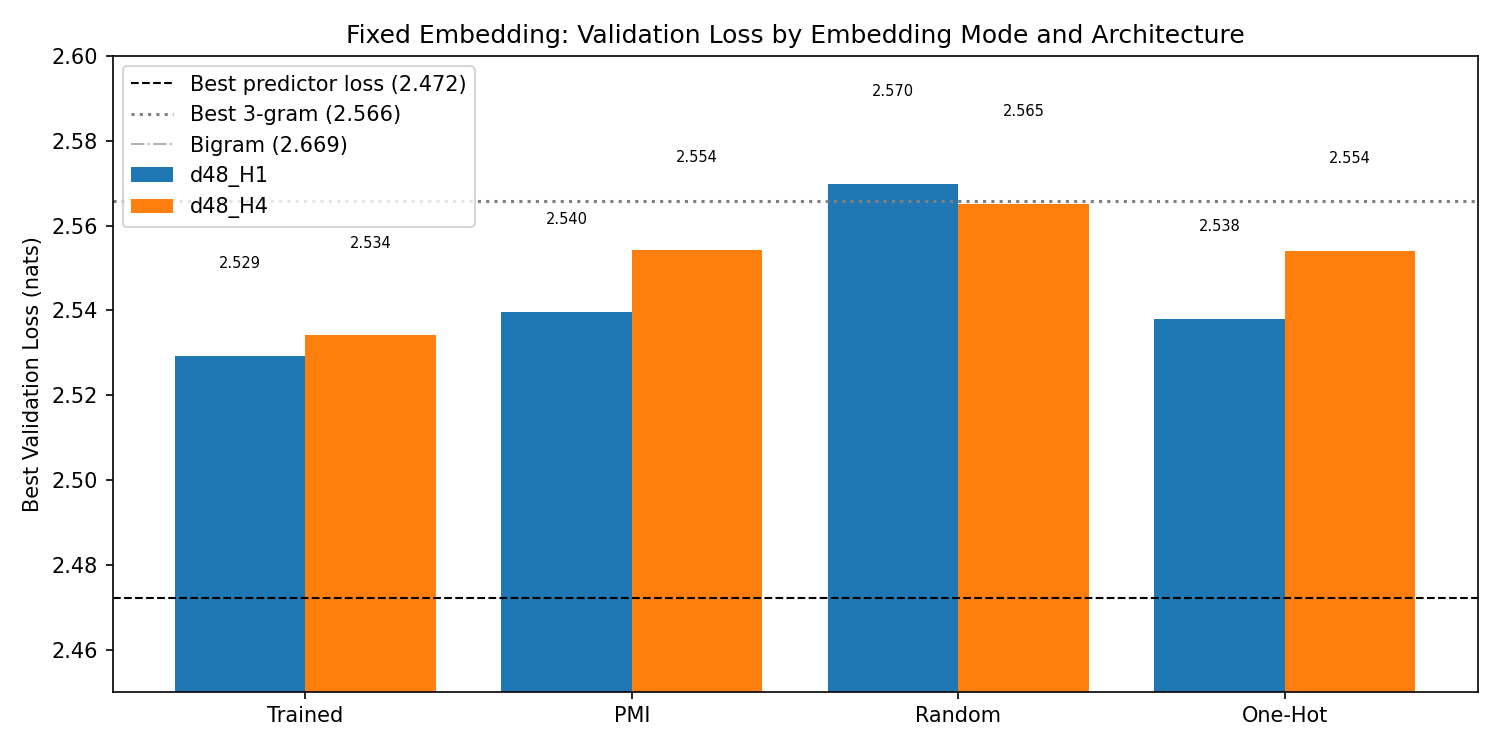
\includegraphics[width=\textwidth]{fixed_embedding_comparison.png}
  \caption{Best validation loss (nats/token) by embedding initialisation
           and model size.  At $d{=}48$, all embedding modes converge to
           nearly the same loss (${\approx}\,2.47$), close to the
           Bayes-optimal bound.  At smaller $d$, the \texttt{trained} and
           \texttt{pmi} embeddings substantially outperform
           \texttt{random}, \texttt{coulomb}, and
           \texttt{sparse\_binary}, indicating that embedding geometry is
           critical when model capacity is limited.}
  \label{fig:fixed-emb}
\end{figure}

Table~\ref{tab:fixed-emb} reports the numerical values.

\begin{table}[htbp]
  \centering
  \begin{tabular}{l r r r}
    \toprule
    Embedding mode & $d{=}8$, $H{=}1$ & $d{=}16$, $H{=}1$ & $d{=}48$, $H{=}4$ \\
    \midrule
    \texttt{trained}       & 2.849 & 2.614 & 2.474 \\
    \texttt{pmi}           & 2.893 & 2.859 & 2.474 \\
    \texttt{coulomb}       & 3.560 & 3.061 & 2.476 \\
    \texttt{random}        & 3.580 & 3.057 & 2.476 \\
    \texttt{sparse\_binary}& 3.687 & 3.055 & 2.504 \\
    \midrule
    Entropy rate $h$       & \multicolumn{3}{c}{$\approx 2.44$ nats} \\
    \bottomrule
  \end{tabular}
  \caption{Best validation cross-entropy (nats/token) for each
           embedding mode and model configuration.  All models use
           $L = 4$ layers, full architecture, no LayerNorm.}
  \label{tab:fixed-emb}
\end{table}

The results confirm the predictions from Section~3:
the \texttt{trained} embedding performs best at every scale, followed
by \texttt{pmi}.  The three structure-agnostic embeddings
(\texttt{random}, \texttt{coulomb}, \texttt{sparse\_binary}) cluster
together and lag significantly at $d{=}8$ and $d{=}16$.  At $d{=}48$,
the model has enough capacity to compensate for any embedding geometry,
and all modes converge to within $0.03$\,nats of each other.

%----------------------------------------------------------------------
\section{Usage}
%----------------------------------------------------------------------

All experiments use the standard \texttt{base\_config.yaml} (4 layers,
$d = 8$, 1 head, full architecture, no LayerNorm).  Run each condition
with:

\begin{verbatim}
python src/train_fixed_embedding.py --embedding_mode <mode>
\end{verbatim}

For the \texttt{trained} condition, additionally pass
\texttt{-{}-checkpoint\_path models/cylinderhmm/<run>/best\_model.pt}.

\end{document}
